\section{Hierarchical clustering and ordered heatmaps}
\label{sec:clustering}

\subsection{Ordered heatmaps}

RMT decomposes the correlation matrix into spectral components, while ordered heatmaps provide a visual diagnostic of whether these components display block-like organization. Figure~\ref{fig:ordered_heatmaps} orders the assets through hierarchical clustering and displays original, filtered and group-mode structures. The purpose is exploratory and diagnostic: the heatmaps assess whether spectral filtering is associated with patterns that can be interpreted in relation to sector and subsector classifications.

The original matrix displays a broad positive background, consistent with the large leading eigenvalue. The filtered matrix preserves part of this organized dependence while reducing the contribution of eigenvalues inside the random-matrix band. The group-mode matrix has lower average correlation by construction, but its ordered representation displays localized block-like patterns that are less dominated by the market-wide component.

\begin{center}
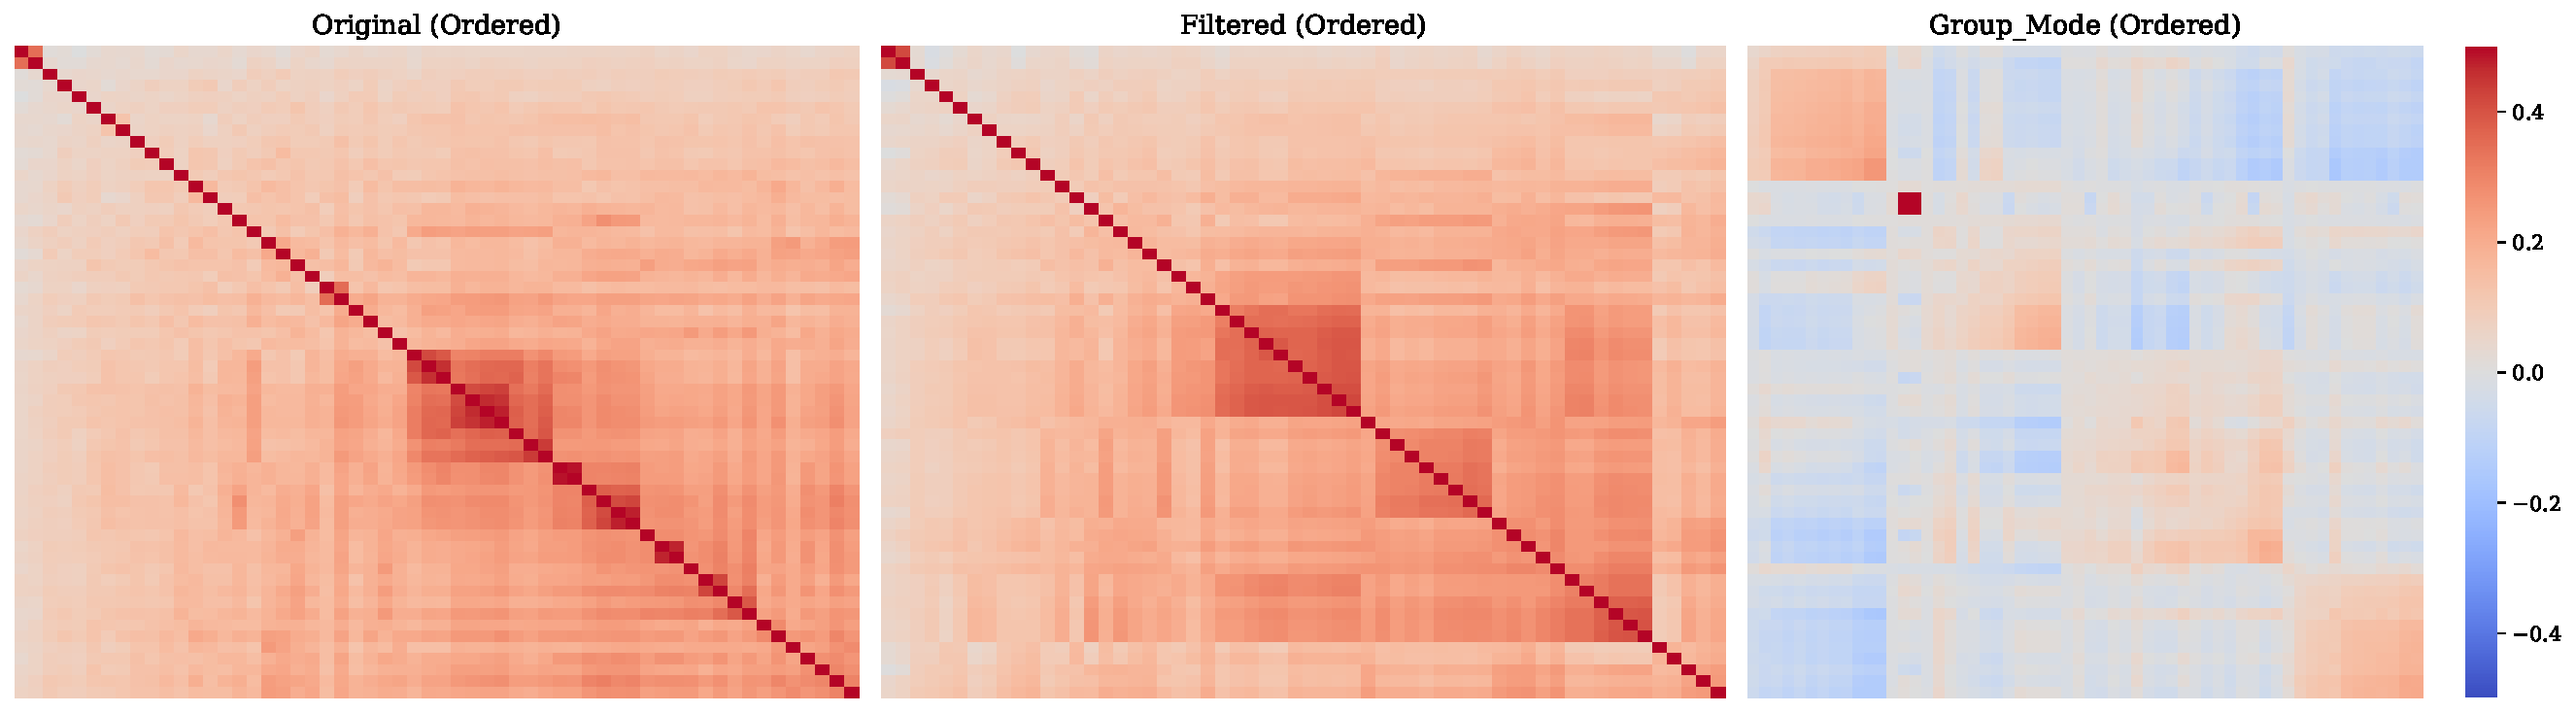
\includegraphics[
  width=\linewidth,
  height=0.72\textheight,
  keepaspectratio
]{images/figure_10_ordered_heatmaps.pdf}
\captionof{figure}{Ordered heatmaps for original and RMT-filtered correlation matrices. Hierarchical ordering reveals block structures that are less visible in unordered matrices.}
\label{fig:ordered_heatmaps}
\end{center}

\subsection{Dendrograms comparison}

Dendrograms provide a complementary view of the same distance geometry. Figure~\ref{fig:dendrograms} compares hierarchical clustering trees for original, filtered and group-mode matrices. These trees help identify which assets merge at shorter distances and how the hierarchy changes after market-mode removal. Branch stability is not formally tested here; the dendrograms are used as exploratory summaries of the distance geometry.

\begin{center}
\captionof{table}{Cophenetic correlations for hierarchical clustering.}
\label{tab:cophenetic_summary}
\begin{tabular}{lrr}
\toprule
Matrix & Assets & Cophenetic correlation \\
\midrule
Original & 58 & 0.9500 \\
Filtered & 58 & 0.9340 \\
Group Mode & 58 & 0.8705 \\
\bottomrule
\end{tabular}
\end{center}

The cophenetic correlation is highest for the original matrix, 0.9500, and remains high for the filtered matrix, 0.9340. The group-mode value is lower, 0.8705. This decline is expected because removing the leading market component reduces the smooth common structure that is easier to summarize hierarchically. The lower value should therefore be interpreted as evidence that the group-mode distance geometry is less tree-like, not as evidence that it is uninformative.




\begin{center}
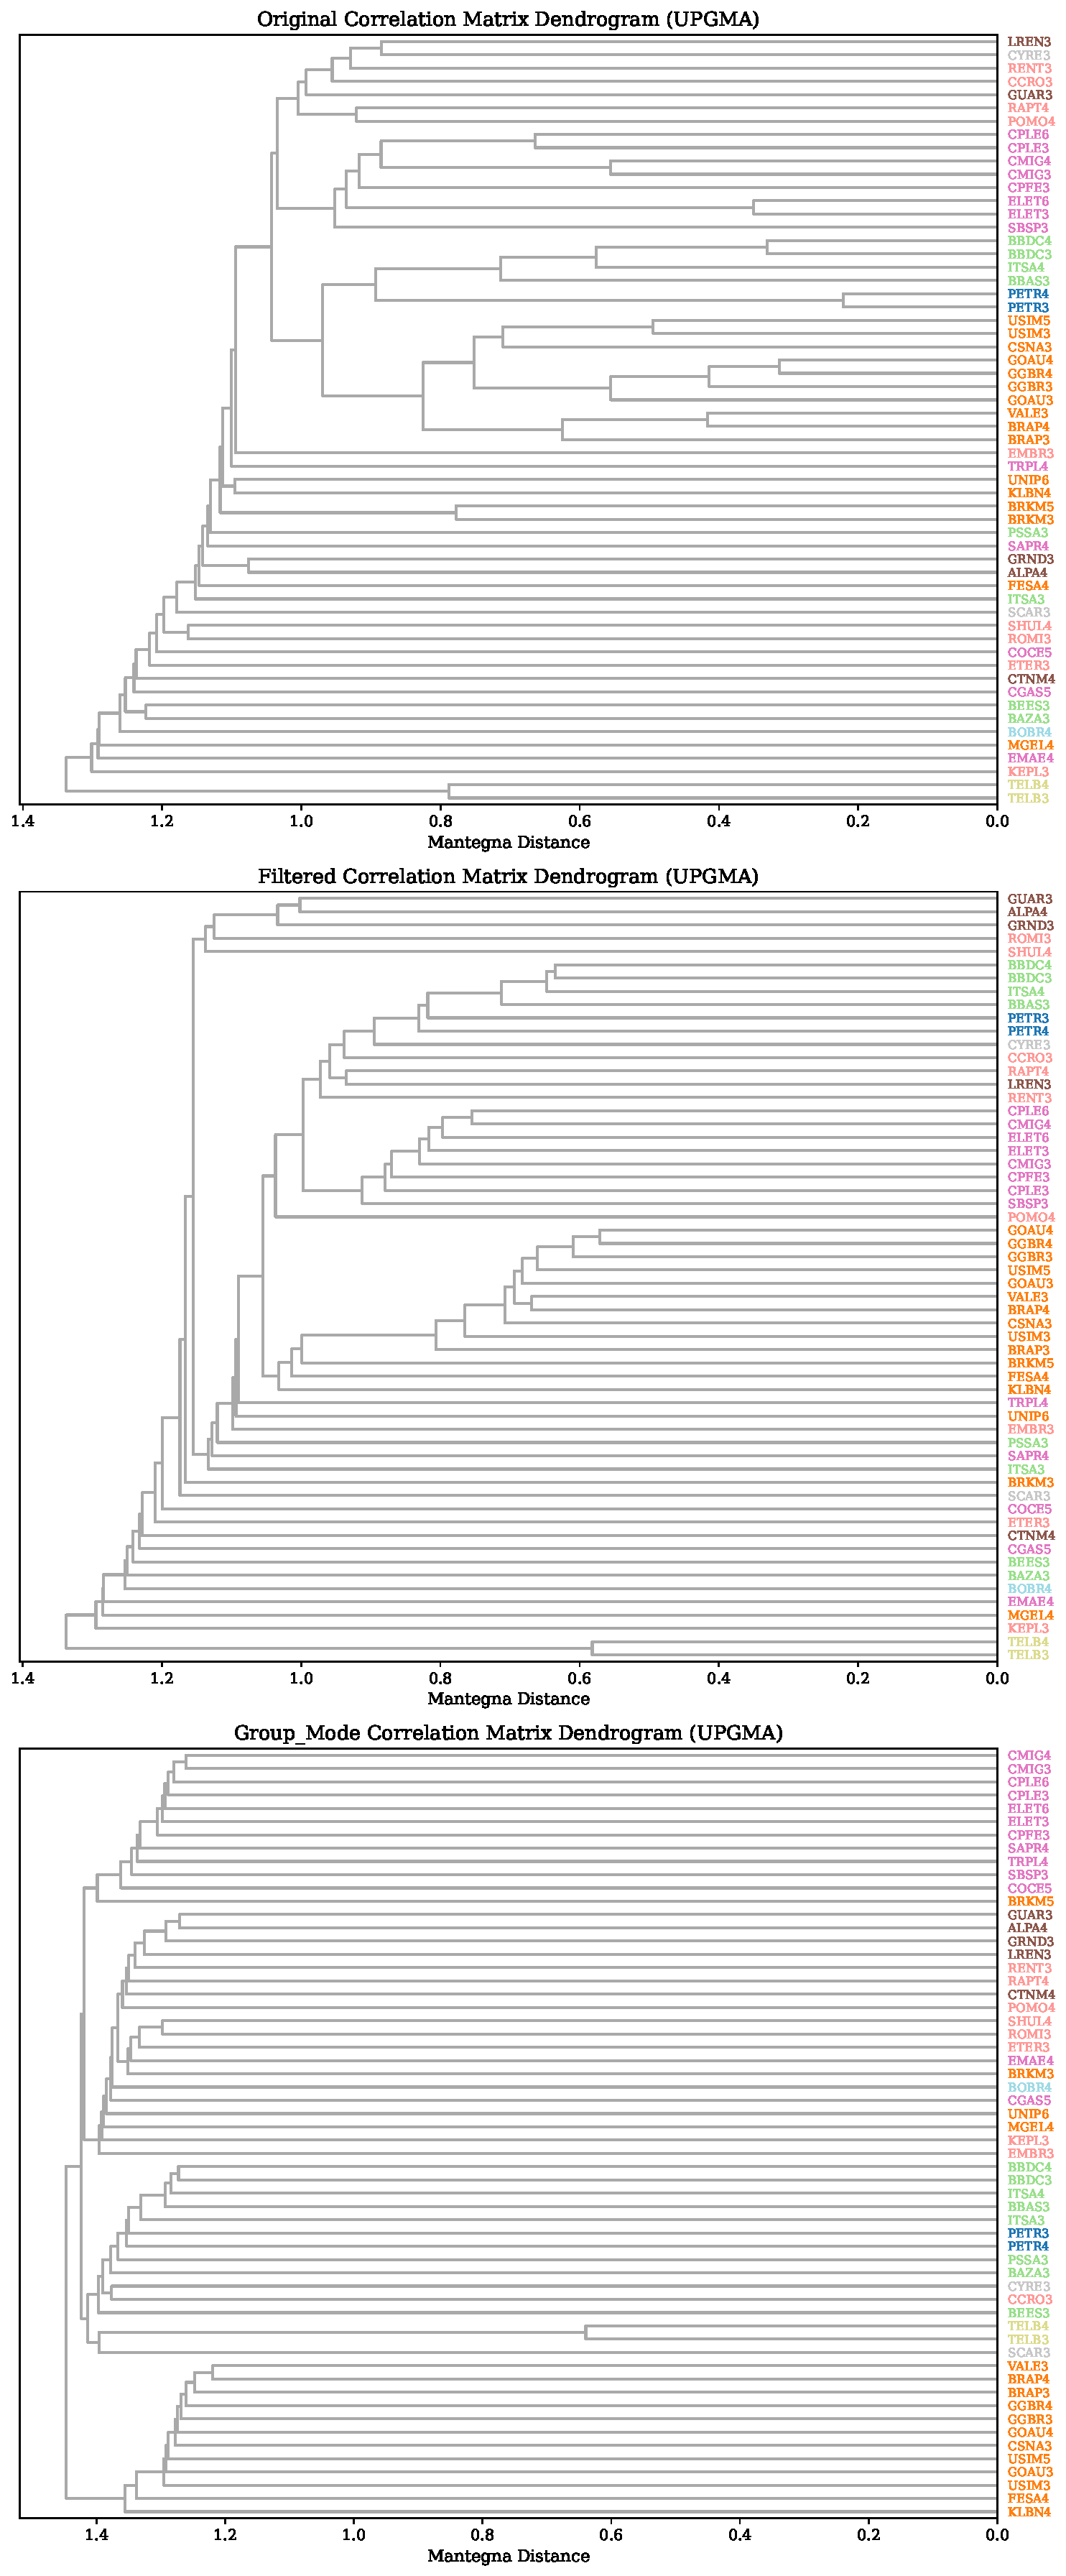
\includegraphics[
  width=\linewidth,
  height=0.8\textheight,
  keepaspectratio
]{images/figure_9_dendrograms_comparison.pdf}
\captionof{figure}{Dendrogram comparison for original, filtered and group-mode matrices using Mantegna distances and average linkage.}
\label{fig:dendrograms}
\end{center}

The clustering results connect naturally to network filtering. Ordered heatmaps and dendrograms suggest that localized structure remains after RMT filtering. The next section examines how this structure appears when only the strongest distance-ranked edges are retained under MST and PMFG constraints.